  
\documentclass[12pt]{article}
\usepackage[utf8]{inputenc}
\usepackage[brazil]{babel}
\usepackage{hyphenat}
\usepackage{graphicx}
\usepackage{amsmath}
\graphicspath{{images/}}
\usepackage{float}

% ---- Capa
\title{%
    Modelagem de Sistemas Dinâmicos\\ % \\ pula linha
    \large Trabalho 3}
\author{Erica da Cunha Ferreira }
\date{Novembro 2020}
\begin{document}
\maketitle
\pagenumbering{gobble} 
\vspace{8cm} %5mm vertical space
\begin{center}
    
\includegraphics[width=0.2\textwidth]{logo.png}
\end{center}

%-----Sumário
\newpage
\tableofcontents
\newpage
\pagenumbering{gobble} 

%---- Pág 1
\cleardoublepage\pagenumbering{arabic}
\section{Introdução}

\quad Este trabalho tem como objetivo analisar um satélite modelado por uma modelo multivariável de 3 entradas e 3 saídas. Estas variáveis controladas são as velocidades angulares (3D) do satélite que são estabilizadas a zero em tempo infinito.

\section{Metodologia}

\quad É disponibilizado 2 arquivos para este trabalho, sta\underline{\hspace{.05in}}control\underline{\hspace{.05in}}satellite.stlx e sta\underline{\hspace{.05in}}control\underline{\hspace{.05in}}satellite\underline{\hspace{.05in}}simu.m, sendo o diagrama de blocos do sistema e o código do Matlab, respectivamente.

\quad No arquivo sta\underline{\hspace{.05in}}control\underline{\hspace{.05in}}satellite\underline{\hspace{.05in}}simu.m, temos as seguintes incógnitas e seus valores. 

\begin{itemize}

    \begin{equation*}
        \lambda = eig(J)
    \end{equation*}
    
    \begin{equation*}
        \lambda_m = min(\lambda)
    \end{equation*}
    
    \begin{equation*}
        \lambda_M = max(\lambda)
    \end{equation*}
    
    \begin{equation*}
        \omega_o = [-0.0021; -0.0067; 0.0253]
    \end{equation*}
    
    \begin{equation*}
        \delta_1 = 1 + \frac{\lambda_M}{\lambda_m}
    \end{equation*}
    
    \begin{equation*}
        \delta_2 = 0
    \end{equation*}
    
    \begin{equation*}
        k_1e = \sqrt{(2\delta_2)}
    \end{equation*}
    
    \begin{equation*}
        k_1 = 1
    \end{equation*}
    
    \begin{equation*}
        K_2e = 2\delta_1
    \end{equation*}
    
    \begin{equation*}
        k_2 = 6.8728
    \end{equation*}
    
    \begin{equation*}
        k_3e = max\left(3\delta_2 + \frac{2\delta_2^2}{{k_1}^2}, \frac{9(k_1 \delta_1)^2}{16k_2(k_2 - 2\delta_1)} + \frac{0.5 k_1^2\delta_1 -2k_1^2k_2+ k_2\delta_2}{k_2 - 2\delta_1}\right)
    \end{equation*}
    
    \begin{equation*}
        k_3 = 1
    \end{equation*}
    
    \begin{equation*}
        \beta_1 = \left(1.5k_1^2k_2 + 1\delta_2k_2\right)^2
    \end{equation*}
    
    \begin{equation*}
        \beta_2 = k_3k_l^2 - 1\delta_2^2 - 3\delta_2k_1^2
    \end{equation*}
    
    \begin{equation*}
        \alpha_1 = \frac{\frac{9}{16}(k_1\delta_1)^2(k_2 + 0.5\delta_1)^2}{k_2}
    \end{equation*}
    
    \begin{equation*}
        \alpha_2 = k_2(k_3 + 2k_1^2 - \delta_2) - (2k_3 + 0.5k_1^2)\delta_1   - \frac{9(k_1\delta_1)^2}{16k_2}
    \end{equation*}
     
    \begin{equation*}
         k_4e = max\left(\frac{\beta_1}{\beta_2} + 2k_2^2 + 1.5k_2\delta_1, \frac{\alpha_1\left((k_2-2 \delta_1) + (2k_2^2 \delta_1 + 0.25k_2 \delta_1^2)\right)}{\alpha_2(k_2-2\delta_1}\right)
     \end{equation*}
      
     \begin{equation*}
        k_4 = k_4e   
     \end{equation*}
     
\end{itemize}

\quad No arquivo sta\underline{\hspace{.05in}}control\underline{\hspace{.05in}}satellite.stlx, temos o seguinte diagrama de blocos, que representa o sistema.

\begin{figure}[H] 
    \centering
    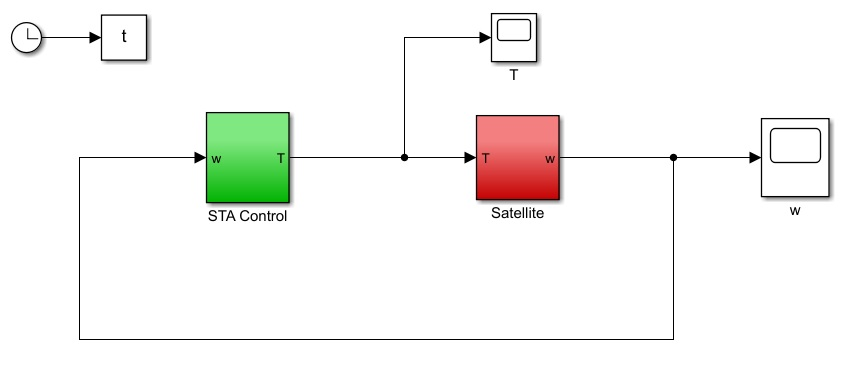
\includegraphics[width=.9\textwidth]{fig3.jpg}
    \caption{Diagrama de Blocos do Sistema}
\end{figure}

\quad Ao clicar no \emph{STA Control}, temos o seguinte diagrama de blocos que representa o sistema.

\begin{figure}[H] 
    \centering
    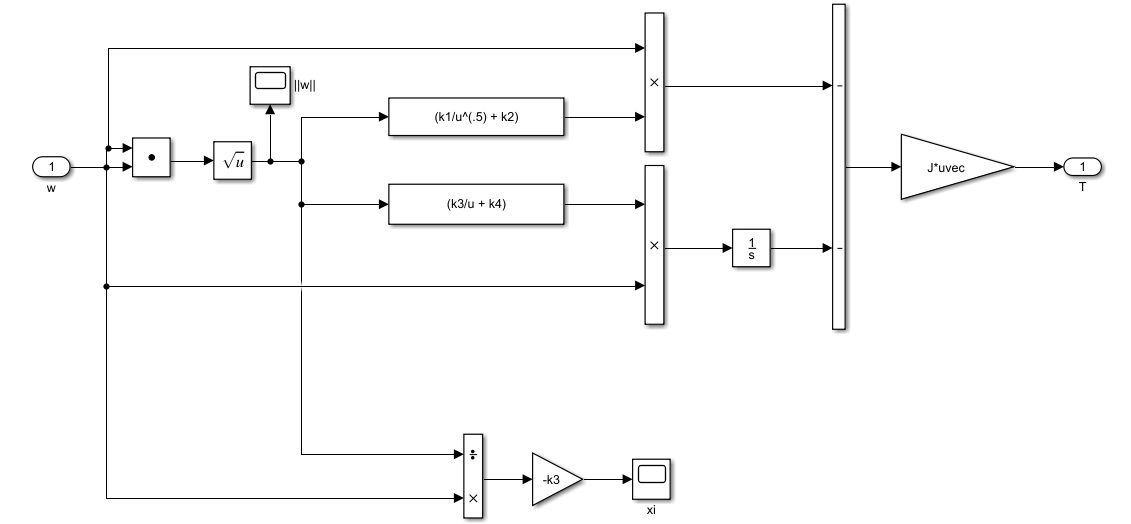
\includegraphics[width=0.9\textwidth]{fig1.jpg}
    \caption{Diagrama de Blocos STA Control}
\end{figure}

\quad Abaixo, estão expostas as respectivas equações obtidas a partir do diagrama de blocos acima: 


\begin{equation}
    \beta_1 = \omega x \left(\frac{k_1}{\sqrt{u_1}}\right) + k_2
\end{equation}

\begin{equation}
   \dot{\beta_2} = \omega x \left(\frac{k_3}{\sqrt{u_1}}\right) + k_4 
\end{equation}

\begin{equation}
    \beta = \beta_1 + \beta_2 
\end{equation}  

\begin{equation}
    u_1 = \sqrt{\vec{\omega} \cdot \vec{\omega} }
\end{equation}  

\begin{equation}
    T = J \times \beta_{vec} 
\end{equation}

\begin{equation}
    x_i = \frac{-(k_3 \times \omega)}{u_1} \cdot 
\end{equation}

\quad Ao clicar no bloco \emph{Satellite} da \textbf{Figura 1}, temos o seguinte diagrama de blocos:

\begin{figure}[H] 
    \centering
    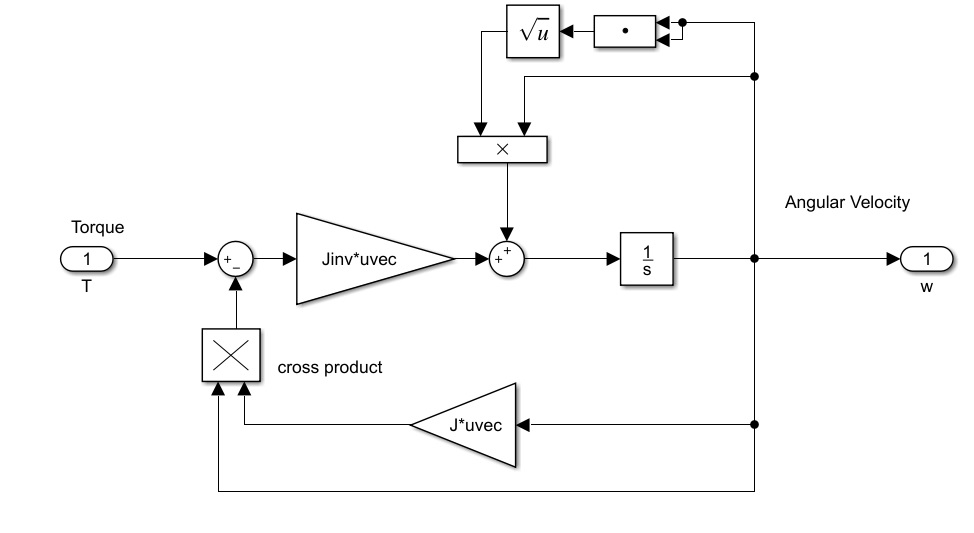
\includegraphics[width=0.9\textwidth]{fig2.jpg}
    \caption{Diagrama de Blocos Satellite}
\end{figure}

Abaixo estão as equações a partir do diagrama de blocos do \emph{Satellite}:

\begin{itemize}

    \begin{equation}
        \alpha = T - J \times \omega_{vec} \times \omega_{vec}
    \end{equation}
    
    \begin{equation}
        \dot{\omega} = J_{inv}\alpha_{vec} + \left(\vec{\omega} \cdot \vec{\omega} \times \sqrt{\omega}\right) \times \sqrt{\omega}
    \end{equation}
\end{itemize}

\quad Ao clicar no \emph{scope} chamado de T, temos a seguinte imagem, nela podemos observar que o torque se estabiliza em zero.

\begin{figure}[H] 
    \centering
    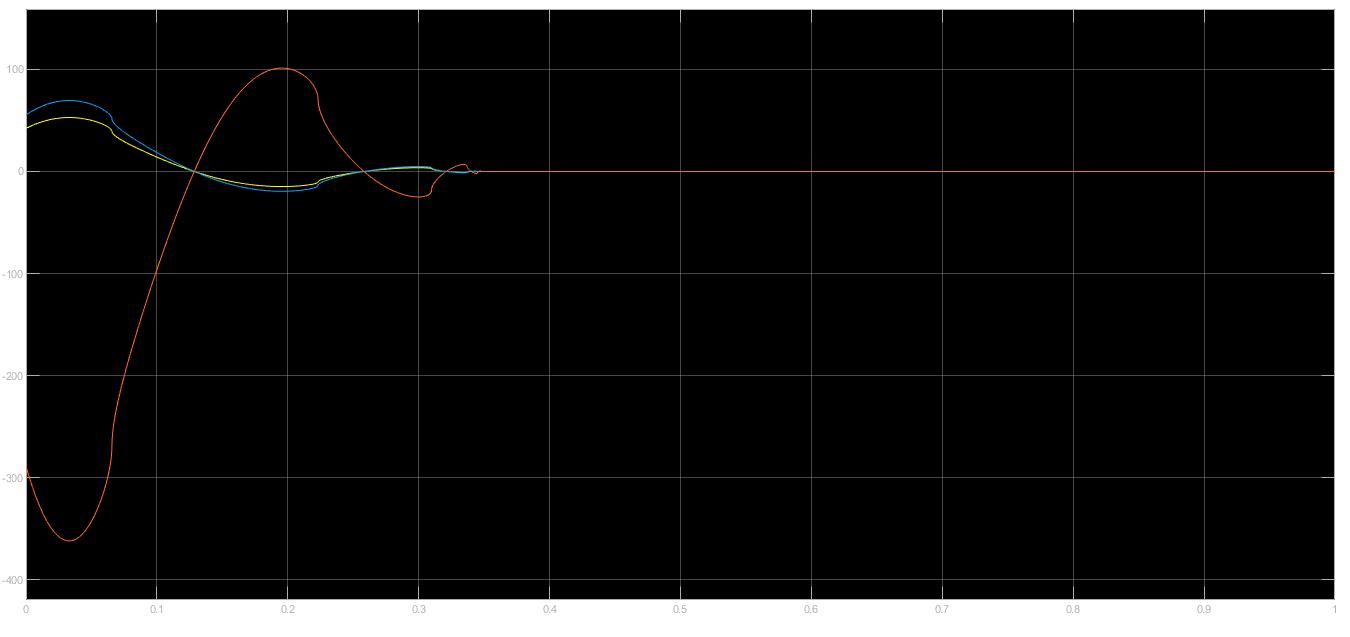
\includegraphics[width=0.8\textwidth]{T, entrada.jpg}
    \caption{Diagrama do Bloco T}
\end{figure}

Como resultado final do programa sta\underline{\hspace{.05in}}control\underline{\hspace{.05in}}satellite\underline{\hspace{.05in}}simu.m, temos o seguinte gráfico:

\begin{figure}[H] 
    \centering
    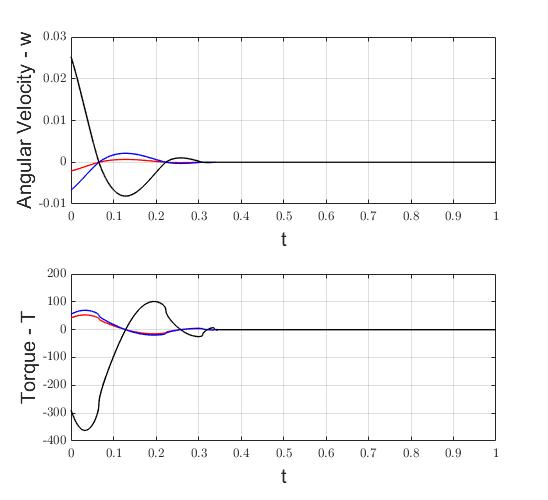
\includegraphics[width=.7\textwidth]{trab 4 matlab1.jpg}
    \caption{Código Simulado}
\end{figure}

\quad Ao analisar a saída de Velocidade angular, é possível ver que as respostas traçadas indicam sobrepasso período de tempo compreendido entre 0.16 segundos e 0.22 segundos. Ainda, quando t =
0.32 segundos, todas as respostas assentam-se em y = 0.
Analisando a saída b, temos sobrepassos e 0.13, 0.25 e 0.32
segundos. Ainda, quando t = 0.34 segundos, o assentamento ocorre para o valor de y = 0.

\section{Conclusão}

\begin{figure}[H] 
    \centering
    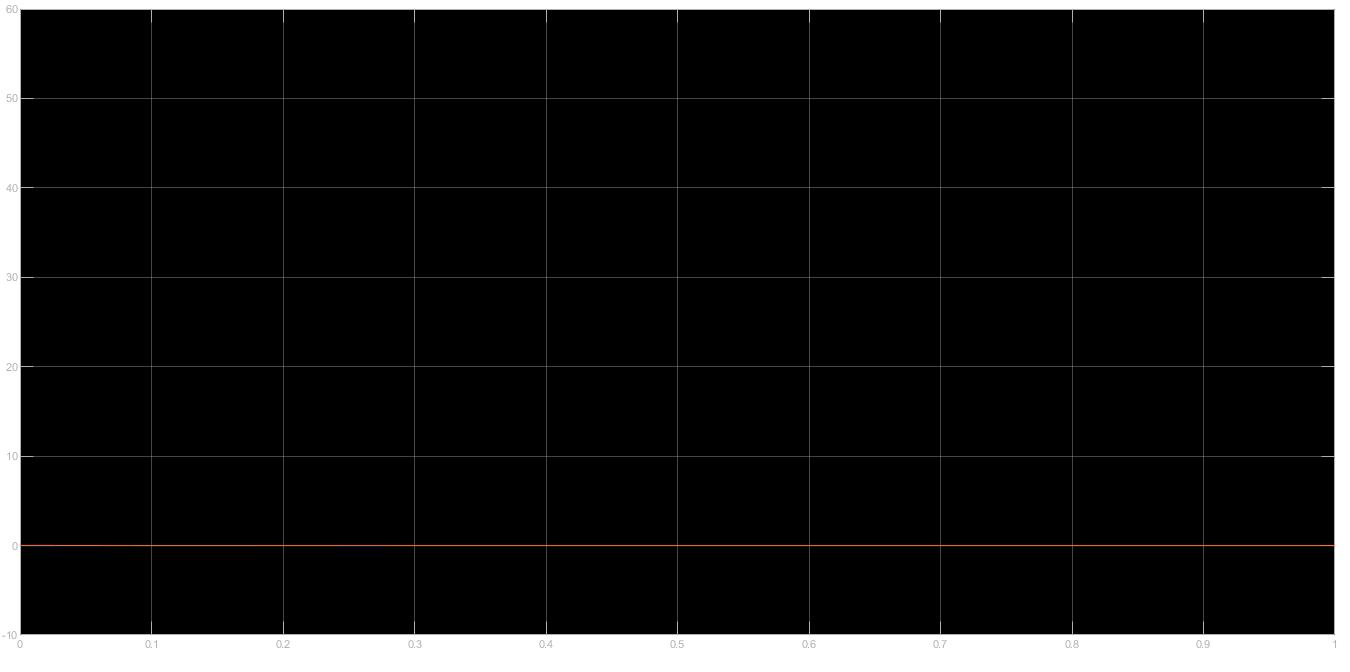
\includegraphics[width=.7\textwidth]{trab 4 matlab2.jpg}
    \caption{Resultado do Sistema}
\end{figure}

\quad Como pode ser observado nas \textbf{Figuras 4,5,6}, o código atinge com sucesso o seu objetivo, de estabilizar as velocidades angulares utilizando o torque, uma vez que como podemos ver na \textbf{Figura 6}, que mostra a representação final do sistema, temos todas as velocidades tendendo a zero.

\end{document}
